\documentclass[twocolumn]{report}

%Encoding
\usepackage[T1]{fontenc}
\usepackage[utf8]{inputenc}

%Typography
\usepackage{microtype}
\usepackage{parskip}
\usepackage{libertine}
\usepackage[libertine]{newtxmath}

%Technical
\usepackage[version=4]{mhchem}
\usepackage{isotope}
\usepackage{siunitx}
\usepackage{mathrsfs,amsmath}
\DeclareSIUnit\permil{\text{\textperthousand}}

%Enumeraton
\usepackage{acronym}
\usepackage{array}
\usepackage{enumitem}

%Graphics
\usepackage{bmpsize}
\usepackage[dvipdfmx]{graphicx}
\usepackage{endiagram}
\usepackage{tikz}
\usepackage{wrapfig}
\usetikzlibrary{shapes.geometric}
\usetikzlibrary{decorations.pathreplacing}
\tikzset{every picture/.style=semithick}

%Referencing
\usepackage[colorlinks]{hyperref}
\usepackage{cleveref}

%Title
\title{Ocean Notes}
\author{\href{mailto:hgpa2018@mymail.pomona.edu}{Henry Peterson}}
\date{\today}

\input{ocean_commands}

%Body
\begin{document}
\maketitle
\tableofcontents
\chapter{The Coriolis Effect}\label{coriolis}

The Coriolis Effect is foundational to the study of the ocean and atmosphere. The largest dynamical features of Earth's surface---atmospheric cells, surface currents, thermohaline circulation, etc.---are all influenced by this effect, which is characterized by the following:
\begin{enumerate}
	\item motion at Earth's surface is \emph{deflected} to the right in the northern hemisphere and to the left in the southern hemisphere.
	\item the effect appears as acceleration which is proportional ($\propto$) and perpendicular ($\perp$) to velocity.\footnote{Equivalently, as a force which is proportional and perpendicular to momentum.}
	\item the effect is greatest at the poles and \num{0} at the equator
	\item the radius of curvature for such a deflected object is proportional to its velocity; slow motion curves more tightly than fast motion
\end{enumerate}
We will start with a brief overview of the relevant mathematical constructions used to describe the Coriolis effect. \href{https://www.youtube.com/playlist?app=desktop&list=PLZHQObOWTQDPD3MizzM2xVFitgF8hE_ab}{\textcolor{blue}{This playlist}} is recommended for further information on the math.
\section{Vector}
A vector is a mathematical object which encodes both \emph{direction} and \emph{magnitude}. Magnitude may be a unitless number or a quantity (the product of a number and a set of units). Direction is usually determined relative to some position, but vectors in general do not retain this position information. We will see how this plays out later.

Here, vectors are drawn as arrows with magnitude represented by length (although the true meaning may have nothing to do with length) and tails placed at the origin. Vectors pointing toward or away from the reader are drawn as a circled dot (arrowhead) or cross (tail feathers), respectively. See Figure \ref{vectors}.

\begin{figure}
\begin{center}
    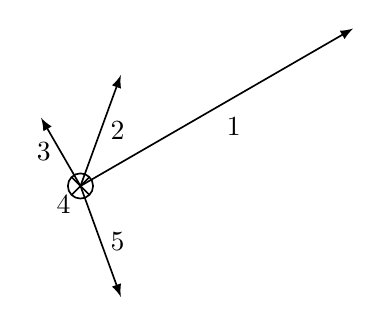
\begin{tikzpicture}
	\draw[-latex] (0,0) -- node [below right]{\vecv{1}} (30:4);
	\draw[-latex] (0,0) -- node [right]{\vecv{2}} (70:1.5);
	\draw[-latex] (0,0) -- node [left]{\vecv{3}} (120:1);
	\draw[-latex] (0,0) -- node [right]{\vecv{5}} (-70:1.5);
    \draw (0,0) circle (.16) node [below left]{\vecv{4}};
    \foreach \x in {0,...,3}
		\draw (0,0) -- +(45+\x*90:.16);
  	\end{tikzpicture}
  	\end{center}
	\caption{Geometric representation of vectors.}
	\label{vectors}
	\end{figure}
Some quantities are easier to conceptualize as vectors than others. For example, acceleration imposed by gravity at Earth's surface is given by the vector \vg\ with downward direction and magnitude: 
\begin{equation}
||\vg||\approx\qty{9.8}{\m\per\second\squared}\label{g}
\end{equation}
Earth's angular velocity $\av$ takes a bit more imagination to imagine as a vector. Its magnitude (angular \emph{speed}) is the angular distance travelled per unit time, which is characteristically uniform for a rigid rotating object. We know that every point will travel once around the circle over the period $T$, so we have:
\begin{equation}
||\av||=2\pi/T
\end{equation}
On Earth $T$ is the sidereal day \qty{86164}{\second}:
\begin{equation}
||\Omega||=2\pi/\qty{86164}{\second}\approx\qty{7.29e-5}{\per\second}\label{omega}
\end{equation}
and its direction is parallel to Earth's axis of rotation, i.e., from Earth toward Polaris.

\section{Cross Product}
The cross product of two vectors $\va\times\vb$ is a third vector $\vc$ which obeys the following rules, summarized visually in Figure \ref{crossproduct}:
\begin{enumerate}
    \item The output magnitude $||\vc||$ is the ``area'' of a parallelogram with sides \va\ \& \vb:
	\begin{equation}
	||\vc||=||\va||\cdot||\vb||\cdot\sin\theta\label{mag}
	\end{equation}
The units of this ``area'' need not be length squared, just as the units of a vector need not be length. Notice that holding direction of \va\ and \vb\ constant, scaling $||\va||$ or $||\vb||$ up or down scales $||\vc||$ by the same amount.
    \item \vc\ is perpendicular $(\perp)$ to both \va\ and \vb. If \va\ and \vb\ are two spokes of a wheel, \vc\ is the axle. Thus holding $||\va||$ and $||\vb||$ constant, changing the direction of either \va\ or \vb\ affects \emph{both magnitude and direction} of \vc. $||\vc||$ is greatest when $\va \perp \vb$; $||\vc|| = 0$ when \va\ is parallel to \vb.\label{perp}
    \item Of the two vectors with these properties, \vc\ follows a ``right-hand rule,'' which we will see later.
\end{enumerate}
\begin{figure}
\begin{center}
    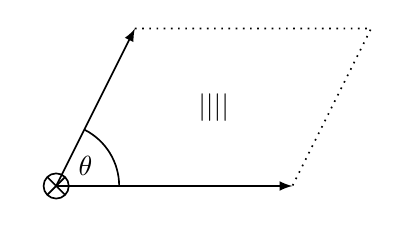
\begin{tikzpicture}
    \draw[white](1,2) --node[black]{$||\vc||$} (3,0);
    \draw[latex-latex](1,2)--node[left]{\va}(0,0)node[above right]{\hspace{.45em}$\theta$} --node[below]{\vb}(3,0);
    \draw[dotted] (1,2) -- (4,2) -- (3,0);
    \draw (.8,0) arc (0:63:.8);
    \draw (0,0) circle (.16) node[left]{$\vc\ $};
    \foreach \x in {0,...,3}
		\draw (0,0) -- +(45+\x*90:.16);
  	\end{tikzpicture}
  	\end{center}
	\caption{Geometric representation of $\va\times\vb=\vc$.}
	\label{crossproduct}
	\end{figure}

\section{Definition}
The Coriolis effect is an apparent force which influences the motion of objects relative to the spinning Earth. We now have the tools necessary to define its mathematical form, although the derivation of this form will not be covered here:
\begin{equation}
    \vCf=-2m\av\times\vV\label{Cf}
\end{equation}
where the Coriolis \emph{force} $\vCf$ depends on the mass $m$ and velocity $\vV$ (relative to Earth) of the moving object.
Alternatively, any force expressed as a function of mass $m$ can be given as an acceleration which is independent of mass:
\begin{equation}
    \vCa=-2\av\times\vV\label{Ca}
\end{equation}
where \vCa\ is Coriolis \emph{acceleration}. The properties of the Coriolis effect follow directly from the the cross product and vector definitions:
\begin{enumerate}
    \item Fundamentally, $\vCa$ is influenced by Earth's rotation and the object's velocity, but not its position.
    \item The amount of acceleration is greatest when $\vV$ is perpendicular to the axis of rotation; it is zero when $\vV$ is parallel.
    \item Coriolis acceleration is always perpendicular to the velocity of the moving object which means things deflect along a curved path but never speed up or slow down.
\end{enumerate}

\section{Example Calculation}
Consider a penguin flying horizontally above the North Pole at speed $||\vV||=\qty{100}{\meter\per\second}$. Notice that $\vV\perp\av\ (\theta=\ang{90})$. How much Coriolis acceleration will it experience? From \cref{omega,mag,Ca}:
\begin{multline*}
||\vCa||=-2\left(\qty{100}{\meter\per\second}\right)\left(\qty{7.29e-5}{\per\second}\right)\sin\ang{90}\\\approx\qty{-0.0146}{\meter\per\second\squared}
\end{multline*}
So the exceptionally fast penguin drifts with an acceleration almost than \num{700} times smaller than that imposed by gravity. If our penguin has a mass of \qty{20}{\kg}, it feels a slight nudge of:
\begin{equation*}
||\vCf||=\qty{20}{\kg}\left(\qty{-0.0146}{\meter\per\second\squared}\right)\approx\qty{-0.29}{\newton}
\end{equation*}
which is roughly the weight of a pencil.

\section{Constraints}
Imagine a big box on a smooth ($\mu_k=0.05$) ice rink. The vertical gravitational (and normal) force $\vg_f=m\cdot\vg$ is \num{20} times greater than horizontal friction $\textbf{f}=\mu_k\cdot m\cdot\vg$. So the box may slide horizontally with a gentle nudge but cannot be lifted easily. That is, vertical motion is limited more than horizontal motion. While a force may come from any direction, only the horizontal component of that force is translated into acceleration.
 
The ocean and atmosphere have analogous dimensional (rather than frictional) constraints. Atmospheric convection takes place primarily in the troposphere, which is \qty{\approx10}{\km} thick. Ocean surface currents occur in the top \qty{\approx100}{\m}; deep circulation is bounded by the abyssal plain \qtyrange{4}{6}{\km} below the surface. By contrast, the ocean and atmosphere each span at least a majority of the Earth's \qty{\approx5.1e8}{\km} surface area in the horizontal dimension. As we have seen, (and will soon quantify) Coriolis deflection is simply not noticeable at the scales involved in vertical motion. This means we only observe \vCah, the horizontal component of \vCa. How do we solve for \vCah?

The relationship between the horizontal plane and $\av$ varies across Earth's surface. At the poles, they are perpendicular; at the equator, parallel. This is why the observable Coriolis effect varies with latitude $(\varphi)$, despite any mention of position in \cref{Cf}. For our flying penguin at the North Pole $(\varphi=\ang{90})$, horizontal motion is always perpendicular to $\av$ and thus the full magnitude of the Coriolis Effect is observed. Compare this to the more complicated situation at the equator $(\varphi=\ang{0})$.

If the penguin flies due North or South at the equator, $\vV\parallel\av$ and thus $||\vCa||=0$. What about East or West? If the penguin continues to fly at \qty{100}{\meter\per\second}, and $\vV\perp\av$, it experiences the same \vCa\ as it did at the pole. But here the direction of \vCa\ is vertical; it is overpowered by gravity and does not cause horizontal drift. Instead, it adds or subtracts to the other acceleration vector in the vertical direction---\vg---and the penguin's \emph{weight} changes imperceptibly. Thus we have two distinct reasons why no Coriolis effect is observed at the equator.

Any direction of \vV\ intermediate between N/S and E/W results in \vCa\ intermediate between the two extremes given. At this location and speed, magnitude varies from $\qtyrange{0}{2.31e-3}{\meter\per\second\squared}$ but direction is always vertical, so $\vCah=0$.

\section{Latitude $(\varphi)$}

What about at latitudes between the poles and equator? Consider a diatom floating in the surface ocean at $\varphi=\ang{30}$. If \vVn\ is due North, the angle $\theta$ between $\vV$ and $\av$ is \ang{30}, that is, $\varphi=\theta$ (see Figure \ref{Vn}).
\begin{figure}
\begin{center}
\begin{tikzpicture}
	%Cross section and latitude
    \draw (0,0) -- (\er,0) arc (0:90:\er) -- cycle;
    \draw (0,0) -- ++(30:\er);
	\draw[dotted] (30:\er) -- ++(-60:1.5);
    %Angles
	\draw (.8,0) arc (0:30:.8);
	\path +(15:.6) node {$\varphi$};
	\draw (0,.8) arc (90:120:.8);
	\path +(105:.6) node {$\theta$};
	%Vectors
	\draw[red,-latex] (30:\er) ->node[right,midway]{\vVn} +(120:1.5);
	\draw[red,-latex] (0,0) ->node[left,midway]{\vVn} +(120:1.5);
	\draw[green!50!black] (30:\er) circle (.1) node[right]{$\vCa=\vCah$};
	\foreach \x in {0,...,3}
		\draw[green!50!black] (30:\er) -- +(45+\x*90:.1);
	\draw[blue,-latex] (0,0) ->node[right]{$\av$} ++(0,3.2);
  	\end{tikzpicture}
\caption{$\varphi=\theta$ for due-North motion}
\label{Vn}
\end{center}
\end{figure}

If \vVs\ is due South, $\theta$ is the supplement of $\varphi\ (\ang{180}-\varphi=\theta)$. Note that $||\vCa||$ ($\propto$ area) is identical in both cases (see Figure \ref{Vns}).
\begin{figure}
\begin{center}
    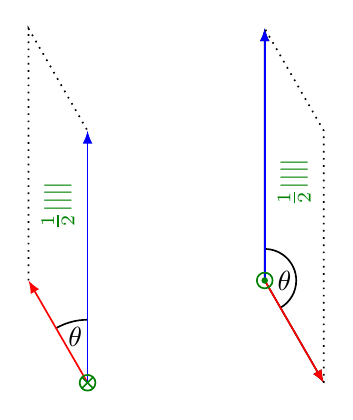
\begin{tikzpicture}
    \draw[white](0,3.2) ++(120:1.5) --node[green!50!black,rotate=90]{$\frac{1}{2}||\vCah||$} (0,0);
    \draw (0,.8) arc (90:120:.8);
    \path (0,0) ++(105:.6) node {$\theta$};
    \draw[red,-latex] (0,0) ->node[left,midway]{\vVn} ++(120:1.5);
    \draw[blue,-latex] (0,0) ->node[right]{$\av$} ++(0,3.2);
    \draw[dotted](0,0) ++(120:1.5) -- ++(90:3.2) -- ++(-60:1.5);
    
    \draw[green!50!black] (0,0) circle (.1) node[right]{$\vCah$};
	\foreach \x in {0,...,3}
		\draw[green!50!black] (0,0) -- +(45+\x*90:.1);
    
    \draw[white](3,3.2) ++(120:1.5) --node[green!50!black,rotate=90]{\phantom{mm}$\frac{1}{2}||\vCah||$} (3,0);
    \draw (3,.4) ++(120:1.5) arc (90:-60:.4);
    \path (3,0) ++(120:1.5) ++(0:.25) node {$\theta$};
    \draw[latex-latex](3,0) -- ++(120:1.5) -- ++ (0,3.2);
    \draw[red,latex-] (3,0) -- node[left,midway]{\vVs} ++(120:1.5);
    \draw[blue,-latex] (3,0) ++(120:1.5) ->node[left]{$\av$} ++(0,3.2);
    \draw[dotted](3,0) -- ++(0,3.2) -- ++(120:1.5);
    
    \draw[green!50!black] (3,0) ++(120:1.5) circle (.1) node[left]{$\vCah$};
	\filldraw[green!50!black] (3,0) ++(120:1.5) circle (.03);
		
  	\end{tikzpicture}
	\caption{Equivalence of $||\vCah||$ for due-North ($\varphi=\theta$) and due-South ($\varphi=\ang{180}-\theta$) motion.}
	\label{Vns}
  	\end{center}
	\end{figure}

Thus we can substitute $\sin\varphi$ for $\sin\theta$ as we calculate $||\vCah||$ for North/South motion:

\begin{gather}
||\vCa||=2\cdot||\vV||\cdot||\av||\cdot\sin\theta\nonumber\\
||\vCa||=||\vCah||=2\cdot||\vV||\cdot||\av||\cdot\sin\varphi\label{vCah_ns}
\end{gather}

What about East-West motion? Like the situation at the poles and equator, $\vV\perp\av$, so $||\vCa||$ is mathematically identical to what it would be at the poles. The difference here is that the direction of \vCa\ now includes a vertical component which is not observed. Unlike at the equator, \vCa\ now also includes a horizontal component, which is observed. Figure \ref{Vew} shows that we \emph{must} include a factor of $\sin\varphi$ in our definition of \vCah\ for East/West motion. Since $\vV\perp\av$, we have $\sin\theta=1$, thus: 

\begin{gather}
||\vCa||=2\cdot||\vV||\cdot||\av||\cdot1\nonumber\\
||\vCah||=2\cdot||\vV||\cdot||\av||\cdot\sin\varphi\tag{\ref{vCah_ns}}
\end{gather}

\begin{figure}
\begin{center}
\begin{tikzpicture}
	%Cross section and latitude
    \draw (0,0) node[left]{A.} -- (\er,0) arc (0:90:\er) -- cycle;
    \draw (0,0) -- ++(30:\er);
    %Angles
	\draw (.8,0) arc (0:30:.8);
	\path +(15:.6) node {$\varphi$};
	\draw (-.8,0) ++ (30:\er) ++ (2,0) arc (180:210:.8);
	\path ++ (30:\er) ++ (2,0) ++(195:.6) node {$\varphi$};
	
	\draw[thin, dotted] (30:\er) -- ++(120:1.5);
	\draw[thin, dotted] (30:\er) -- ++(-60:1.5);
	\draw[ultra thin] (30:\er) +(-60:1) --node[below,sloped]{\vCav} +(2,0);
	%Vectors
	\draw[-latex] (30:\er) ->node[above,midway]{$\vCa$} +(2,0);
	\draw[green!50!black,-latex] (30:\er) ->node[below,sloped]{$\vCah$} +(-60:1);
	\draw[red] (30:\er) circle (.1) node[above]{\vVe\ };
	\foreach \x in {0,...,3}
		\draw[red] (30:\er) -- +(45+\x*90:.1);
	\draw[blue,-latex] (0,0) ->node[left]{$\av$} ++(0,3.2);
  	\end{tikzpicture}
	\begin{tikzpicture}
	%Cross section and latitude
    \draw (0,0) node[left]{B.} -- (\er,0) arc (0:90:\er) -- cycle;
    \draw (0,0) -- ++(30:\er);
    %Angles
	\draw (.8,0) arc (0:30:.8);
	\path +(15:.6) node {$\varphi$};
	\draw (.8,0) ++ (30:\er) ++ (-2,0) arc (0:30:.8);
	\path ++ (30:\er) ++ (-2,0) ++(15:.6) node {$\varphi$};
	
	\draw[thin, dotted] (30:\er) -- ++(120:1.5);
	\draw[thin, dotted] (30:\er) -- ++(-60:1.5);
	\draw[ultra thin] (30:\er) +(120:1) --node[above,sloped]{\vCav} +(-2,0);
	%Vectors
	\draw[-latex] (30:\er) ->node[below left]{$\vCa$} +(-2,0);
	\draw[green!50!black,-latex] (30:\er) ->node[above,sloped]{$\vCah$} +(120:1);
	\draw[red] (30:\er) circle (.1) node[right]{\vVw};
	\filldraw[red] (30:\er) circle (.03);
	\draw[blue,-latex] (0,0) ->node[left]{$\av$} ++(0,3.2);
  	\end{tikzpicture}
\caption{$||\vCah||=||\vCa||\cdot\sin\varphi$ for due-East (A.) and due-West (B.) motion.}
\label{Vew}
\end{center}
\end{figure}

So we find that despite North/South and East/West motion influencing \vCah\ very differently, the expression for $||\vCah||$ is concisely expressed for all horizontal directions a function of $\varphi$, not $\theta$. For completeness, we can give an expression for the vector \vCah\ as a product of $||\vCah||$ and a unit vector \vu\ with a subscript indicating the vector to which \vu\ is perpendicular ($\vu\perp\vV$ in both cases):
\begin{gather}
\vCa=2\cdot||\vV||\cdot||\av||\cdot\sin\theta\cdot\vu_\Omega\\
\vCah=2\cdot||\vV||\cdot||\av||\cdot\sin\varphi\cdot\vu_\vg\label{Cah}
\end{gather}
\section{Curvature $(\kappa)$}
We want to know how velocity and acceleration interact to shape the path travelled by a Coriolis-affected object. The relevant parameter is curvature, defined by $\kappa=1/R$, where $R$ is the radius of curvature. In general:
\begin{equation}
\kappa=\frac{||\vV\times\va||}{||\vV||^3}
\end{equation}
where $\va$ is the acceleration vector.\footnote{\href{https://web.ma.utexas.edu/users/m408m/Display13-4-3.shtml}{Derivation}} For a Coriolis-affected object, the $\va$ of interest is \vCah, and since $\vV\perp\vCah$, we can define Coriolis curvature:
\begin{equation}
\kappa_C=\frac{||\vV||\cdot||\vCah||\cdot\sin\ang{90}}{||\vV||^3}=\frac{||\vCah||}{||\vV||^2}
\end{equation}
Or, recalling from \cref{Cah} that $||\vV||$ is a factor of $||\vCah||$, we can skip the \vCah\ calculation altogether:
\begin{multline}
\kappa_C=\frac{2\cdot||\vV||\cdot||\av||\cdot\sin\varphi}{||\vV||^2}\\
=\frac{2\cdot||\av||\cdot\sin\varphi}{||\vV||}
\end{multline}
For a calculation with more practical meaning, we take the reciprocal to find the radius of curvature:
\begin{equation}
	R=\frac{||\vV||}{2\cdot||\av||\cdot\sin\varphi}
\end{equation}
For one practical example, assume the Gulf Stream current has a maximum surface speed \qty{2.5}{\meter\per\second}. At $\varphi=\ang{30}$:
\begin{multline}
R=\frac{\qty{2.5}{\meter\per\second}}{2\left(\qty{7.29e-5}{\per\second}\right)\cdot\sin\ang{30}}\\
\approx\qty{34}{\km}
\end{multline}
Since the actual gulf stream is part of the North Atlantic subtropical gyre (which is much larger than \qty{34}{\km} in radius) we can see that the Coriolis force is not the only force at play in shaping the complex dynamics of ocean circulation. For instance, what causes the current to begin flowing in the first place? Nonetheless, it's important to develop some intuition for magnitude of the effects involved in the Coriolis effect in this simplified example.
\section{Which Way?}
Another angle from which to approach the Coriolis effect gives an intuitive answer to the last big question we have put off to this point: which of the two directions is correct? We know $\vCah\perp\vV$ and $\vCah\perp\vg$, so from the perspective of the moving object, it must be either left or right.

Consider a ``stationary'' ($\vV=0$) iceberg at the equator. Of course, it isn't really stationary because it is moving along with the ground beneath as the Earth rotates (and orbits, etc. but we consider here the reference point of a \emph{non-rotating} object orbiting the sun alongside Earth). The Earth's circumference is roughly \qty{40000}{\km}, and it rotates once in a day (that's the period $T$ we saw in the definition of angular velocity \ref{omega}), so the iceberg is traveling at a blistering \qty{450}{\m\per\second}, faster than the speed of sound, relative to the nearby observer. If the iceberg has mass (it does) then it carries a non-zero momentum\footnote{This velocity $v$ is \emph{not} the same as \vV, becuase \vV\ is relative to the Earth's spinning reference frame.} $p=mv$ which it tends to maintain (Newton's first law of motion).

Imagine the iceberg begins to drift toward the North Pole, carrying its equator-derived momentum as it goes. As it drifts, it finds the Earth appears to move slower than it once did, approaching a point at the pole where there is no motion at all, only rotation fixed in place. Still holding on to all its momentum, the iceberg drifts in the direction of the Earth's rotation---to the East (from the iceberg's North-bound perspective, to the right). If the iceberg were to drift South again from the pole, it would experience the opposite effect. Now the Earth is moving faster relative to its original stationary momentum, so it lags behind the rotation. Now, it drifts west, which is again to the right. By symmetry, deflection is to the left in the southern hemisphere.

East/West motion is a bit trickier. If the iceberg drifts eastward, it begins to outpace the Earth's rotation. As it speeds up, it is flung outward---like an elastic cord stretching out as it is whipped in a faster circle. But since this drift isn't strong enough to overcome gravity, it simply causes a slow drift toward the equator, the latitude with the greatest distance from the axis of rotation. Likewise, westward drifting causes a slower speed and a drift toward the poles, the closest spot to the rotation axis.

\chapter{Acids \& Bases}\label{acidbase}
Liquid water partially dissociates into \ce{H+} and \ce{OH-} ions:
\[\ce{H2O(l) <=>[K_w] H+(aq) + OH-(aq)}\]
At equilibrium, the molar concentrations (denoted by square brackets) of these ions are related to the auto-ionization constant \ce{K_w}:
\begin{equation}
    \ce{K_w = [H+][OH^-]}=\qty{e-14}{M\squared}\label{kw}
\end{equation}
In neutral water, the concentration of each species is balanced:
\begin{equation}
    \ce{[H+] = [OH^-]}=10^{-7}M\label{neut}
\end{equation}
Acids and bases disrupt \eqref{neut} such that \ce{[H+] \neq [OH^-]} by donating or accepting protons, respectively. However, they do not ultimately alter the equilibrium relation \eqref{kw}. This is important because it means \ce{[H+]} and \ce{[OH-]} are totally dependent on one another; the entire system can be characterized by only one variable. pH is the most commonly used parameter:
\[\ce{pH=-\log[H+]}\]
\section{Conjugate Pairs}
Acids and bases come in \textit{conjugate pairs.} After an acid donates a proton, the remaining species is a conjugate base. After a base accepts a proton, it becomes a conjugate acid.
\section{Strong \& Weak Species}
Strong acids and bases participate in proton exchange more readily than weak ones. The strength of conjugate pairs is inverse, i.e., a strong acid has a weak conjugate base and vice versa.
For example, nitric acid is a strong acid which readily donates its proton into solution, setting up an unbalanced equilibrium:
\[\ce{HNO3 <=>> H+ + NO3^-}\]
Since nitric acid is so effective at donating its proton, the conjugate base \ce{NO3^-} is very weak and does not act as an effective base. By contrast, weak species like carbonic acid set up more balanced equilibria:
\[\ce{H2CO3 <=> H+ + HCO3-}\]
The conjugate base \ce{HCO3-} is strong enough participate in proton exchange and thus qualifies as a base. The distinction between strong and weak species allows us to proceed with a definition of Alkalinity.
\chapter{Inorganic Carbon Cycle}\label{carbonate}
\section{Equilibria}
The atmospheric concentration of carbon dioxide (\ce{pCO2}) is a primary factor influencing global climate today and through deep time. The oceanic inorganic carbon reservoir is over 50 times that of the atmosphere, so atmosphere-ocean exchange drives \ce{pCO2} over millennial timescales. The goal of this section is to derive a quantitative model which relates \ce{pCO2} to the measurable ocean carbonate system.

When \ce{CO2} dissolves, it reacts with water to form carbonic acid (\ce{H2CO3^*})\footnote{It is difficult to distinguish between dissolved carbon dioxide and carbonic acid, so they are grouped as a single species}, bicarbonate (\ce{HCO3-}), and carbonate (\ce{CO3^2-}). These reactions are reversible, so the following equilibrium is established:
\begin{multline}
    \ce{CO2 (g) + H2O (l) <=>[K0] H2CO3^* (aq) \\ <=>[K1] H+ (aq) + HCO3- (aq) \\ <=>[K2] 2H+ (aq) + CO3^2- (aq)}\label{sys}
\end{multline}
\ce{K_{0,1,2}} are measurable concentration ratios of reactants by products at equilibrium:
\begin{gather}
    \ce{K0 = [H_2CO_3^{*}]/pCO_2}\label{K0}\\
    \ce{K1 = [H^+][HCO_3^-]/[H_2CO_3^*]}\label{K1}\\
    \ce{K2 = [H^+][CO_3^{2+}]/[HCO_3^-]}\label{K2}
\end{gather}
Dissolved Inorganic Carbon (DIC) and Alkanility (Alk) are also measurable:
\begin{multline}
    \ce{DIC = \underset{0.5\%}{[H_2CO_3^*]} + \underset{88.6\%}{[HCO_3^-]} + \underset{10.9\%}{[CO_3^{2-}]} \\ \approx [HCO3^-] + [CO3^2-]}\label{DICappx}
\end{multline}
Alk is the charge-balanced\footnote{Concentrations of species which exchange more than one proton are scaled accordingly.} excess of bases in solution, primarily carbonic conjugate bases:
\begin{multline}
     \ce{Alk = \underset{76.8\%}{[HCO_3^-]} + \underset{18.7\%}{2[CO_3^{2-}]} + \\ \underset{4.2\%}{[B(OH)_4^-]} + \underset{0.2\%}{(\Sigma[B] - \Sigma[A])} \\
     \approx [HCO3^-] + 2[CO3^2-]\label{alkc}}
\end{multline}
\section{Derivation}
Rearranging equilibrium constant expressions gives:
\begin{gather}
    \ce{[H+] = K2.[HCO3^-]/[CO3^2-]}\tag{\ref{K2}}\\
    \ce{[H2CO3^*] = [H+][HCO3^-]/K1}\tag{\ref{K1}}\\
    \ce{pCO2 = [H_2CO_3^{*}]/K_0}\tag{\ref{K0}}
\end{gather}
Sequential substitution and simplification gives:
\begin{equation}
    \ce{pCO2 = \frac{K2}{K0.K1}\cdot\frac{[HCO3^-]^2}{[CO3^{2-}]}}\label{CO2K}
\end{equation}
Subtracting~\eqref{alkc} from \eqref{DICappx} and substituting the result back into \eqref{DICappx} gives:
\begin{gather}
    \ce{[CO3^2-] \approx Alk - DIC}\\
    \ce{[HCO3^2-] \approx $2$DIC - Alk}
\end{gather}
Finally, substituting back into~\eqref{CO2K} gives:
\begin{equation}
\ce{pCO2 \approx \dfrac{\ce{K2}}{\ce{K0\cdot K1}}\cdot \dfrac{(\ce{$2$DIC - Alk})^2}{\ce{Alk - DIC}}}
\end{equation}
\section{Calcium}
The complexity of the carbonate system leads to some counter-intuitive dynamics. One of these is the observation that an increase in \ce{[H2CO3^*]} has the effect of \textit{lowering} \ce{[CO3^2-]}. To understand why, recall from \eqref{sys}:
\[\ce{H2CO3}^{*}\ce{<=>[K1] H+(aq) + HCO3^-(aq)}\]
By Le Chatelier's principle, increasing the concentration of the reactant \ce{H2CO3^*} will shift the reaction to the right, and thus more \ce{H+} and \ce{HCO3-} will be produced in equal measure, say by amount a. Next, consider how this increase affects the balance of the next equilibrium \eqref{sys}:
\begin{equation}
    \ce{HCO3-(aq) <=>[K2] H+(aq) + CO3^2-(aq)}
\end{equation}
Recall that the equilibrium concentrations of the products in this reaction are much lower than the product. Thus, the same increase + a to both sides will have a greater effect on the products, shifting the equation to the left (converting \ce{CO3^2-} to \ce{HCO3-}). With the addition of carbonic acid, carbonate alkalinity is consumed. Or, in terms of the equilibrium constant expression:
\begin{equation}
    \ce{K2 = \dfrac{[H^+][CO_3^{2+}]}{[HCO_3^-]}}\tag{\ref{K2}}
\end{equation}
Solving for \ce{[CO3^2-]}:
\[\ce{[CO3^2-] \propto \dfrac{[HCO3-]}{[H+]}}\gg1\]
Clearly, as a increases with the addition of \ce{H2CO3^*}, \ce{[CO3^2-]} will decrease.
The concentration of carbonate is of key concern in another geochemical system, the biological calcium carbonate pump.

Calcium carbonate forms two minerals, calcite and aragonite, which many ocean organisms use to build shells and exoskeletons.
\[\ce{CaCO3(s) <=>[K_{sol}] Ca^2+(aq) + CO3^2-(aq)}\]
\[\ce{K_{sol}=[Ca^2+][CO3^2-]}\]
\ce{[Ca^2+]} = \qty{10}{\mmol\per\kg}
\\\ce{[CO3^2-]} $\approx$ \qtyrange[range-units = single]{40}{200}{\umol\per\kg}
\chapter{Nitrogen}
\section{Isotope Fractionation}
\newcommand{\dN}{\delta\isotope[15]{N}}
\newcommand{\eps}{\varepsilon}
Nitrogen has two stable isotopes: \isotope[14]{N} and \isotope[15]{N}. Isotopes form the same compounds and participate in the same reactions; both are thus present in any nitrogenous sample. However, many reactions preferentially consume certain isotopes. For some reaction involving N, \ce{K_{14}} and \ce{K_{15}} represent the rate constants for the reactions involving only the respective isotope. The degree to which such a reaction distinguishes between isotopes is given by the isotopic fractionation factor $\alpha$:
\begin{gather}
    \alpha = \ce{K_{15}/K_{14}}\label{alpha}\\
    \eps = \alpha - 1\label{epsilon}
\end{gather}
Most\footnote{The only significant biological reaction which does not fractionate N isotopes is Nitrification, the original source of fixed N forms to the ocean cycle} biological reactions preferentially consume lighter isotopes; thus $\alpha<1$ and $\eps$ is negative. For incomplete reactions,\footnote{Theoretically, all reactions are incomplete, as there is always some reverse reaction. For practical calculations, only systems with measurable pools of substrate and product are considered incomplete.} isotopes are partitioned into pools of substrate (reactant) and product, whose isotope ratios may differ. These variations provide information about the chemical circumstances in which a sample formed, and the degree of completion for the relevant reaction. If we let $R$ indicate the  isotope ratio \isotope[15]{N}/\isotope[14]{N} with atmospheric \ce{N2} serving as a reference:
\begin{equation}
    R_{atm} \approx.003663\label{R}
\end{equation} then the geochemical tracer used to measure N isotope ratios is $\dN$:
\begin{equation}
   \dN=\frac{R}{R_{atm}}-1\label{d15N}
\end{equation}
$\delta\ce{^{15}N}$ and $\eps$ are expressed in parts per thousand (\unit{\permil}). 
\section{Derivation}
\begin{equation}
    \alpha=\dfrac{R_{p(i)}}{R_s}=\frac{\left(\dfrac{d\ce{^{15}N_p}}{d\ce{^{14}N_p}}\right)}{\left(\ce{\dfrac{^{15}N_s}{^{14}N_s}}\right)}=\frac{d\ce{^{15}N_p}}{\ce{^{15}N_s}}\Big/\frac{d\ce{^{14}N_p}}{\ce{^{14}N_s}}\label{alpha/R}
\end{equation}
When $t=0;\ \ce{N_s = N_{s(0)}}$. Some steps involving integrating (?):
\begin{equation}
    \alpha \times \ln{\left(\frac{\ce{^{14}N_s}}{\ce{^{14}N_{s(0)}}}\right)}=\ln{\left(\frac{\ce{^{15}N_s}}{\ce{^{15}N_{s(0)}}}\right)}\label{integrated}
\end{equation}
\begin{equation}
    f = \ce{\frac{N_s}{N_{s(0)}}}\label{f}
\end{equation}
Since \ce{^{14}N} predominates \eqref{R},
\begin{equation}
    f \approx \ce{\frac{^{14}N_s}{^{14}N_{s(0)}}}\label{f_approx}
\end{equation}
Substituting \eqref{f_approx} into \eqref{integrated}:
\begin{align*}
    \alpha \times \ln{f} &=\ln{\left(\frac{\ce{^{15}N_s}}{\ce{^{15}N_{s(0)}}}\right)}\\
    &=\ln{\left(\frac{\ce{^{15}N_s}}{\ce{^{15}N_{s(0)}}}\times\frac{\ce{^{14}N_{s(0)}\times^{14}N_s}}{\ce{^{14}N_s\times^{14}N_{s(0)}}}\right)}\\
    &=\ln{\left[\left(\ce{\frac{^{15}N_s}{^{14}N_s}}\Big/\ce{\frac{^{15}N_{s(0)}}{^{14}N_{s(0)}}}\right)\times\ce{\frac{^{14}N_s}{^{14}N_{s(0)}}}\right]}
\end{align*}
Substituting \eqref{R} and \eqref{f_approx}:
\begin{equation}
    \alpha \times \ln{f} = \ln{\left(\frac{R_s}{R_{s(0)}}\right)}+\ln{f}
\end{equation}
Rearranging and substituting from \eqref{epsilon}:
\begin{gather}
    \eps \times \ln{f} \approx \ln{\left(\frac{R_s}{R_{s(0)}}\right)}\label{epsilon*lnf}\\
    \frac{R_s}{R_{s(0)}}=f^\eps
\end{gather}
From \eqref{d15N}:
\begin{gather}
1+\delta\ce{^{15}N}=\frac{R}{R_{atm.}}\nonumber\\
R=R_{atm.}(1+\delta\ce{^{15}N})
\end{gather}
Substituting into \eqref{epsilon*lnf}:
\begin{align}
    \eps \times \ln{f} &\approx \ln{\left(\frac{R_{atm.}(1+\delta\ce{^{15}N}_s)}{R_{atm.}(1+\delta\ce{^{15}N}_{s(0)})}\right)}\nonumber\\
    &\approx \ln{\left(\frac{1+\delta\ce{^{15}N}_s}{1+\delta\ce{^{15}N}_{s(0)}}\right)}\label{eps.delta15_ratio}
\end{align}
For small values of $u$ and $v$ \eqref{R}:
\[\ln{\left(\frac{1+u}{1+v}\right)}\approx u-v\]
Thus, from \eqref{eps.delta15_ratio}:
\begin{gather}
    \eps \times \ln{f} \approx \delta\ce{^{15}N}_s - \delta\ce{^{15}N}_{s(0)}\nonumber\\
    \eps \approx \frac{\delta\ce{^{15}N}_s - \delta\ce{^{15}N}_{s(0)}}{\ln{f}}
\end{gather}
\section{Fractionation of Pools}
During a typical biological reaction\footnote{For example: \ce{NO3- ->[k] N_{org}}} which preferentially consumes \ce{^{14}N}, nitrogen is partitioned into substrate (s) and product (p) pools. 
Finally:
\begin{equation}
    \alpha = \dfrac{d\ce{^{15}N_p}}{\ce{^{15}N_p}}\Big/\dfrac{d\ce{^{15}N_p}}{\ce{^{14}N_s}}
\end{equation}
During a reaction which fractionates nitrogen isotopes,  $\delta\ce{^{15}N}$ values of each for the two ``pools,'' i.e., the growing product pool and the dwindling substrate pool, will deviate from the initial substrate value ($\delta\ce{^{15}N_{s(0)}}$) as a function of $\eps$ and $f$, the fraction of substrate remaining compared to the initial value:
\begin{align}
    \delta\ce{^{15}N_s}&=\delta\ce{^{15}N_{s(0)}}-\eps\ln{f}\label{d15ns}\\
    \delta\ce{^{15}N_p}&=\delta\ce{^{15}N_{s(0)}}+\eps\Big(\frac{f\ln{f}}{1-f}\Big)\label{d15np}
\end{align}
Since $\eps$ is negative, $\delta\ce{^{15}N}$ will be lower in the product pool (organic nitrogen) and higher in the substrate pool (dissolved \ce{NO3-}), but not by the same amount.
\section{Motivation}
Atlantic Ocean overturning has significantly slowed during the 20th century, evidenced by the observation that the site of NADW formation is the only region of the Earth that is currently cooling.
\chapter{Redox}\label{redox}
\section{Introduction}
Chemical reactions that permanently transfer electrons between species are called ``Reduction–Oxidation" (Redox). For example:
\[\ce{Cu^2+ (aq) + Zn (s) -> Cu (s) + Zn^2+}\]
can be broken into ``half-reactions" involving either reduction:
\[\ce{Cu^2+ (aq) + 2e- -> Cu (s)}\]
or oxidation:
\[\ce{Zn (s) -> Zn^2+ + 2e-}\]
Notice that when the two half-reactions are added together, the 2 electrons appear on both sides and can thus are neither products not reactants of the overall reaction. Some redox reactions can be more difficult to identify, for example:
\[\ce{CO2 (g) -> C_{\text{org.}} + O2 (g)}\]
is a highly simplified expression for photosynthesis where \ce{C_{\text{org.}}} refers to organic carbon of oxidation state 0. In this case, carbon is reduced:
\[\ce{C^4+ + 4e- -> C_{\text{org.}}}\]
and oxygen is oxidized:\footnote{As you might guess from the name, oxygen is almost always the species doing the oxidizing. Redox chemistry is one of countless ways we can understand photosynthesis as a unique and crucial component of life on a habitable planet.}
\[\ce{2O^2- -> O2 + 4e-}\]
Again, adding the half-reactions allows electrons to cancel. \ce{C^4+} and \ce{2O^2-} are simply the components of \ce{CO2} considered individually.
\section{Energy}
Redox reactions involve energy because charged electrons have different electric potential energy depending on their position relative to charged atomic nuclei. This is analogous to massive objects having different gravitational potential energy depending on their position relative to other massive objects. In both cases, measuring absolute potential energy is not practical, so measurements are made relative to chosen references, such as sea level for $\text{PE}_g$, or for $\text{PE}_e$, the energy associated with the following reduction:
\[\ce{2H+ (aq) + 2e- -> H2 (g)}\]
\section{Environmental Parameter}
Just as acid-base conditions can be characterized by the activity of protons:
\[\ce{pH = -log(H+)}\]
redox conditions can be characterized by the activity of electrons:
\[\ce{pe = -log(e-)}\]
To understand how this might be done, consider one half-reaction from the simplified photosynthesis system described above:
\[\ce{C^4+ + 4e- -> C_{\text{org.}}}\]
An equilibrium constant can be defined as follows:
\[\ce{K = \frac{(C_{\text{org.}})}{(C^4+)(e^-)^4}}\]
Rearranging gives:
\[\ce{(e^-)} = \left[\ce{\frac{(C_{\text{org.}})}{K(C^4+)}}\right]^{1/4}\]
Or in general:
\[\ce{(e^-)} = \left[\ce{\frac{(R)}{K(O)}}\right]^{1/n}\]
For the general reduction half-reaction:
\[\ce{O + \textit{n}\,e^- -> R}\]
Thus:
\[\ce{pe} = \left[\frac{1}{n}\right]\left[\log \ce{K}-\log\frac{(R)}{(O)}\right]\]
The most commonly used redox parameter is defined as follows:
\[\ce{Eh = \frac{2.3RT\cdot pe}{F}}\]
Where R is the constant \qty{8.314}{\joule\per\kelvin\per\mol}, T is temperature in \unit{\K}, and the Faraday constant F is the electric charge of a mole of electrons \qty{9.64853e4}{\coulomb\per\mol}. Further simplification shows Eh has units of \unit{\J\per\coulomb} (\unit{\volt}).
\section{Iron Oxidation}
To give an example of a redox reaction with significant real-world consequences, consider Iron, which originally appears at the surface mostly in its reduced \ce{Fe^{2+}} state in mafic minerals like olivine, pyroxenes, and amphiboles. As it weathers in an oxygenated atmosphere or ocean environment, the following reaction takes place.
\begin{align*}
    4[\ce{Fe^2+ &-> Fe^3+ + e-}]\\ + [\ce{O2 + 4e- &-> 2O^2-}]\\ = \ce{4Fe^2+ + O2 &-> 4Fe^3+ + 2O^2-}
\end{align*}
\ce{Fe^{3+}} is highly insoluble in water compared to \ce{Fe^{2+}}, so one consequence of this reaction is that oxidized iron quickly precipitates out of solution, usually before it has a chance to be carried by rivers into the ocean. Mature soils are often rich in oxidized iron, with reduced-iron minerals having long since degraded. Another consequence has to do with the specific minerals that are formed when \ce{Fe^{3+}} is produced, namely, hematite (\ce{Fe2O3}). From our redox reaction, we can see that oxidized iron and reduced oxygen (\ce{O^{2-}}; ``oxide'') are not produced in the correct ratio for hematite. Instead, we need four more oxygen atoms, supplied by water (\ce{OH-})
\[\ce{4Fe^2+ + O2 + 4OH- -> 4Fe^3+ + 6O^2- + 4H+}\]
Notice that alkalinity \ce{(4OH-)} is consumed, and acidity \ce{(4H+)} is produced. Thus, oxidation of iron is associated with the acidification of the surrounding environment. This can have dramatic consequences on local and global environments. For example, mining often exposes large outcrops of iron (some of which will be reduced, i.e., susceptible to oxidation) very rapidly, which can lead to acid-mine drainage. Alternatively, large increase in the amount of free oxygen in an environment already rich in \ce{Fe^{3+}} can have the same effect. This occured on a global scale, during the Great Oxygenation event (~2.5-2.0 Ga), which led to dramatic chemical transformations of the entire fluid earth.
\end{document}